\documentclass[letterpaper,12pt]{article}
\setlength{\headheight}{15pt}
\setlength{\marginparwidth}{0pt}
\setlength{\marginparsep}{0pt} % width of space between body text and margin notes
\setlength{\evensidemargin}{0.125in} % Adds 1/8 in. to binding side of all 
% even-numbered pages when the "twoside" printing option is selected
\setlength{\oddsidemargin}{0.125in} % Adds 1/8 in. to the left of all pages when "oneside" printing is selected, and to the left of all odd-numbered pages when "twoside" printing is selected
\setlength{\textwidth}{6.375in} % assuming US letter paper (8.5 in. x 11 in.) and side margins as above
\raggedbottom
\setlength{\parskip}{\medskipamount}

\usepackage{amsmath, amsthm, amssymb, fancyhdr, enumitem, tikz, pgfplots}
\pagestyle{fancy}
\lhead{MATH350 --- HW4}
\begin{document}
\paragraph{Homogenous Linear Systems with Constant Coefficients}
\[
    x' = Ax
\]
\paragraph{}where $A\in \mathbb{R}^{n\times n}$
\paragraph{}If $n=1, \frac{dx}{dt} = ax$, where $a \ne 0$, and
\[
    x(t) = K e^{at}
\]
\paragraph{}If $a \ne 0, x(t) = 0$ is the only equilibrium solution ($\frac{dx}{dt} = 0$).
\paragraph{}If $a < 0$, all nontrivial solutions approach $x(t) = 0$. $x(t) = 0$ is an
asymptotically stable solution.

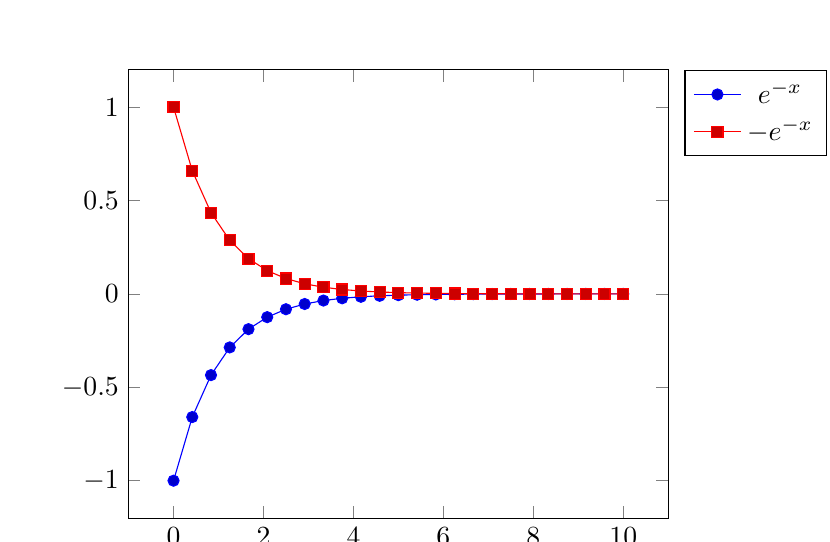
\begin{tikzpicture}
    \begin{axis}[domain=0:10,legend pos=outer north east]
        \addplot {-exp(-x)}; 
        \addplot {exp(-x)};
        \legend{$e^{-x}$, $-e^{-x}$}
    \end{axis}
\end{tikzpicture}
\paragraph{}If $a > 0$, every solution except for the equilibrium solution moves further 
away from $x(t) = 0$. $x(t) = 0$ is an unstable equilibrium solution.

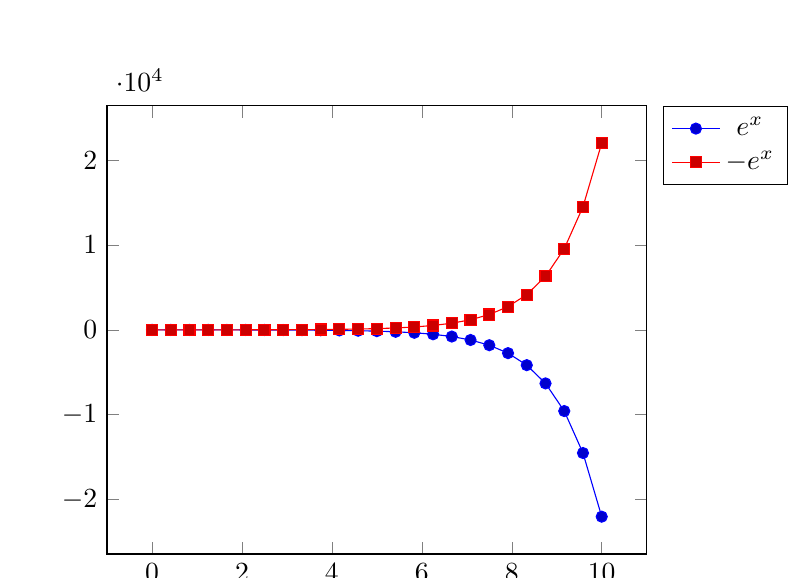
\begin{tikzpicture}
    \begin{axis}[domain=0:10,legend pos=outer north east]
        \addplot {-exp(x)}; 
        \addplot {exp(x)};
        \legend{$e^{x}$, $-e^{x}$}
    \end{axis}
\end{tikzpicture}
\paragraph{Ex:} Find the general solution of

\[
x^{\prime} = 
    \begin{bmatrix}
        2 & 0\\
        0 & -3
    \end{bmatrix}
    x
\]
\begin{align*}
    \begin{bmatrix}
        x_1^{\prime}\\x_2^{\prime} 
    \end{bmatrix}
        &= 
        \begin{bmatrix}
            2x_1 \\ -3x_2
        \end{bmatrix}\\
\end{align*}
\[
    x_1 = C_1e^{2t}\, x_2 = C_2e^{-3t}
\]
\begin{align*}
    x &= \begin{bmatrix}
        C_1e^{2t}\\0
    \end{bmatrix}+
    \begin{bmatrix}
        0\\C_2e^{-3t}
    \end{bmatrix}
    \\
    &= C_1 \begin{bmatrix}
        1\\0
    \end{bmatrix}e^{2t}
    +C_2 \begin{bmatrix}
        0\\1
    \end{bmatrix}e^{-3t}
\end{align*}
\begin{align*}
    W[x^{(1)} \, \, x^{(2)}] &= 
    \begin{vmatrix}
        e^{2t} & 0\\
        0 & e^{-3t}
    \end{vmatrix}\\
                             &= e^{-t}\\
                             &\ne 0
\end{align*}

\paragraph{}Solution of $x^{\prime} = Ax$ has form
\[
    x = \xi e^{rt}
\]
\paragraph{}where the exponent $r$ and the vector $\xi$ must be determined.

\begin{align*}
    x^{\prime} &= r\xi e^{rt}\\
    r\xi e^{rt}  &= A \cdot \xi e^{rt}\\
                r \cdot \xi&= A\cdot \xi\\
                           r \cdot I \cdot \xi&=A\cdot \xi\\
                                              A\xi - rI\xi&= 0\\
                                              (A-rI)\xi&=0\\
\end{align*}

\paragraph{Ex:}Find the general solution of 
\[
    x^{\prime}=
    \begin{bmatrix}
        1&1\\
        4&6
    \end{bmatrix}x
\]
\paragraph{}Assume $x = \xi e^{rt}$.
\begin{align*}
    (A-rI)\xi &= 0\\
    \begin{bmatrix}
        1-r & 1 \\
        4 & 1-r
    \end{bmatrix} 
              \begin{bmatrix}
                  \xi_1\\ \xi_2
              \end{bmatrix}= \begin{bmatrix}
    0\\0
    \end{bmatrix}
\end{align*}
\begin{align*}
    (1-r)^2 - 4 &= 0\\
    1-2r +r^2 -4&= 0\\
    (r-3)(r+1) &= 0
\end{align*}
\paragraph{}$r=3$.
\makeatletter
\renewcommand*\env@matrix[1][*\c@MaxMatrixCols c]{%
\hskip -\arraycolsep
\let\@ifnextchar\new@ifnextchar
\array{#1}}
\makeatother


\[
\begin{bmatrix}[ccc|ccc]
     1& -1 & -1 & 1 & 0 & 0\\
    3 & -1 & 2 & 0 & 1 & 0\\
    2 & 2 & 3 & 0 & 0 & 1\\
\end{bmatrix}
\]
    \[
    \begin{bmatrix}[cc|c]
        -2 & 1 &0\\
        4 & -2 &0
\end{bmatrix}
\] 
\[
    \xi_1^{(1)} = 
    \begin{pmatrix}
        1 \\ 2
    \end{pmatrix}
\]
\[
    \xi_2^{(2)} = 
    \begin{pmatrix}
        1 \\ -2
    \end{pmatrix}
\]
\paragraph{}Thus,

\[
    x^{(1)}= \begin{bmatrix}
        1\\2
    \end{bmatrix}e^{2t}
    \,
    ,
    \,
    x^{(2)}=
    \begin{bmatrix}
        1\\-2
    \end{bmatrix}e^{-t}
\]

\begin{align*}
    W[X^{(1)}\, X^{(2)}] &= \begin{vmatrix}
        e^{3t} & e^{-t}\\
        2e^{3t} & -2e^{t}
    \end{vmatrix}\\
                         &= -2e^{2t} - 2e^{3t}\\
                         &= -4e^{2t}\\
                         &\ne 0
\end{align*}
\paragraph{}Our general solution is 
\begin{align*}
    x &= C_1 x^{(1)}(t) + C_2 x^{(2)}(t)\\
      &=C_1 \begin{bmatrix}
          1\\2
      \end{bmatrix}e^{3t}+
      C_2
      \begin{bmatrix}
          1\\-2
      \end{bmatrix}e^{-t}
\end{align*}

\begin{align*}
    \begin{bmatrix}
        x_1\\x_2
    \end{bmatrix}
    &= 
    \begin{bmatrix}
        C_1e^{3t}+C_2e^{-t}\\
        2C_1e^{3t} - 2C_2e^{-t}
    \end{bmatrix}
\end{align*}
\paragraph{}For large $t$ values, $x_1 \approx C_1 e^{2t}$, and $x_2 \approx 2C_1e^{3t}$, thus,
\begin{align*}
    \frac{x_1}{x_2} &= \frac{1}{2}\\
    x_2 &= 2x_1
\end{align*}
\paragraph{}For large $t$, the first term of each $x_1, x_2$ become dominant, and the
second term becomes negligible. $\to$ All the solutions with non-zero $C_1$ will 
asymptotically approach $x_2 = 2x_1$ as $t \to \infty$.
\end{document}



